% vim: set ts=4 sw=4 tw=80 noexpandtab:

\documentclass{42-en}

%******************************************************************************%
%                                                                              %
%                                   Prologue                                   %
%                                                                              %
%******************************************************************************%
\usepackage[
    type={CC},
    modifier={by-nc-sa},
    version={4.0},
]{doclicense}
\usepackage{amsmath} % The amsmath package provides commands to typeset matrices with different delimiters. 
\usepackage{epigraph}
\setlength\epigraphwidth{.95\textwidth}
\usepackage{multirow}
\usepackage{cancel}
%****************************************************************%
%                  Re/definition of commands                     %
%****************************************************************%

\newcommand{\ailogo}[1]{\def \@ailogo {#1}}\ailogo{assets/42ai_logo.pdf}

%%  Redefine \maketitle
\makeatletter
\def \maketitle {
  \begin{titlepage}
    \begin{center}
	%\begin{figure}[t]
	  %\includegraphics[height=8cm]{\@ailogo}
	  
\includegraphics[height=8cm]{assets/42ai_logo.pdf}
	%\end{figure}
      \vskip 5em
      {\huge \@title}
      \vskip 2em
      {\LARGE \@subtitle}
      \vskip 4em
    \end{center}
    %\begin{center}
	  %\@author
    %\end{center}
	%\vskip 5em
  \vfill
  \begin{center}
    \emph{\summarytitle : \@summary}
  \end{center}
  \vspace{2cm}
  %\vskip 5em
  %\doclicenseThis
  \end{titlepage}
}
\makeatother

\makeatletter
\def \makeheaderfilesforbidden
{
  \noindent
  \begin{tabularx}{\textwidth}{|X X  X X|}
    \hline
  \multicolumn{1}{|>{\raggedright}m{1cm}|}
  {\vskip 2mm 
\includegraphics[height=1cm]{assets/42ai_logo.pdf}} &
  \multicolumn{2}{>{\centering}m{12cm}}{\small Exercise : \@exnumber } &
  \multicolumn{1}{ >{\raggedleft}p{1.5cm}|}
%%              {\scriptsize points : \@exscore} \\ \hline
              {} \\ \hline

  \multicolumn{4}{|>{\centering}m{15cm}|}
              {\small \@extitle} \\ \hline

  \multicolumn{4}{|>{\raggedright}m{15cm}|}
              {\small Turn-in directory : \ttfamily
                $ex\@exnumber/$ }
              \\ \hline
  \multicolumn{4}{|>{\raggedright}m{15cm}|}
              {\small Files to turn in : \ttfamily \@exfiles }
              \\ \hline

  \multicolumn{4}{|>{\raggedright}m{15cm}|}
              {\small Forbidden functions : \ttfamily \@exforbidden }
              \\ \hline

%%  \multicolumn{4}{|>{\raggedright}m{15cm}|}
%%              {\small Remarks : \ttfamily \@exnotes }
%%              \\ \hline
\end{tabularx}
%% \exnotes
\exrules
\exmake
\exauthorize{None}
\exforbidden{None}
\extitle{}
\exnumber{}
}
\makeatother

%%  Syntactic highlights
\makeatletter
\newenvironment{pythoncode}{%
  \VerbatimEnvironment
  \usemintedstyle{emacs}
  \minted@resetoptions
  \setkeys{minted@opt}{bgcolor=black,formatcom=\color{lightgrey},fontsize=\scriptsize}
  \begin{figure}[ht!]
    \centering
    \begin{minipage}{16cm}
      \begin{VerbatimOut}{\jobname.pyg}}
{%[
      \end{VerbatimOut}
      \minted@pygmentize{c}
      \DeleteFile{\jobname.pyg}
    \end{minipage}
\end{figure}}
\makeatother

\usemintedstyle{native}

\begin{document}

% =============================================================================%
%                     =====================================                    %

\title{Machine Learning - Module 04}
\subtitle{Regularization}
\author{
  Maxime Choulika (cmaxime), Pierre Peigné (ppeigne), Matthieu David (mdavid)
}
\summary
{
  Today you will fight overfitting!
  You will discover the concepts of regularization and how to implement it into the algortihms you already saw until now.
}
\maketitle
%******************************************************************************%
%                                                                              %
%                        Section usefull ressources                            %
%                          for ML Modules                                      %
%                                                                              %
%******************************************************************************%


\chapter*{Notions and ressources}

\section*{Notions of the module}
Regularization, overfitting. Regularized loss function, regularized gradient descent.  
Regularized linear regression. Regularized logistic regression.

\section*{Useful Ressources}

You are strongly advise to use the following resource:
\href{https://www.coursera.org/learn/machine-learning}{Machine Learning MOOC - Stanford}
These videos are available at no cost; simply log in, select "Enroll for Free", and choose "audit the course for free" in the popup window.
The following sections of the course are pertinent to today's exercises:

\newpage

\subsection*{Week 3: Classification}

\subsubsection*{Classification with logistic regression (already seen on module 03)}
\begin{itemize}
  \item Motivations
  \item Logistic regression
  \item Decision boundary
\end{itemize}

\subsubsection*{Cost function for logistic regression (already seen on module 03)}
\begin{itemize}
  \item Cost function for logistic regression
  \item Simplified Cost Function for Logistic Regression
\end{itemize}

\subsubsection*{Gradient descent for logistic regression (already seen on module 03)}
\begin{itemize}
  \item Gradient Descent Implementation
\end{itemize}

\subsubsection*{The problem of overfitting (New !!!)}
\begin{itemize}
  \item The problem of overfitting
  \item Addressing overfitting
  \item Cost function with regularization
  \item Regularized linear regression
  \item Regularized logistic regression  
\end{itemize}


\emph{All videos above are available also on this \href{https://youtube.com/playlist?list=PLkDaE6sCZn6FNC6YRfRQc_FbeQrF8BwGI&feature=shared}{Andrew Ng's YouTube playlist}, videos from 31 to 36 (already seen on module 03) and 37 to 41 (new !!!).}
%******************************************************************************%
%                                                                              %
%                        Common Instructions                                   %
%                          for Python Projects                                 %
%                                                                              %
%******************************************************************************%

\chapter*{Common Instructions}
\begin{itemize}
  \item The version of Python recommended to use is 3.7, you can
  check the version of Python with the following command: \texttt{python -V}
  
  \item The norm: during this piscine, it is recommended to follow the
  \href{https://www.python.org/dev/peps/pep-0008/}{PEP 8 standards}, though it is not mandatory.
  You can install \href{https://pypi.org/project/pycodestyle}{pycodestyle} which
  is a tool to check your Python code.
  
  \item The function \texttt{eval} is never allowed.
  
  \item The exercises are ordered from the easiest to the hardest.
  
  \item Your exercises are going to be evaluated by someone else,
  so make sure that your variable names and function names are appropriate and civil. 
  
  \item Your manual is the internet.
  
  \item You can also ask questions on the {https://discord.gg/8Vvb6QMCZq}{42AI} discord.
  
  \item If you find any issue or mistakes in the subject please create an issue on \href{https://github.com/42-AI/bootcamp_python/issues}{42AI repository on Github}.  
  
  \item We encourage you to create test programs for your
  project even though this work \textbf{won't have to be
  submitted and won't be graded}. It will give you a chance
  to easily test your work and your peers’ work. You will find
  those tests especially useful during your defence. Indeed,
  during defence, you are free to use your tests and/or the
  tests of the peer you are evaluating.
  
  \item Submit your work to your assigned git repository. Only the work in the
  git repository will be graded. If Deepthought is assigned to grade your
  work, it will be run after your peer-evaluations.
  If an error happens in any section of your work during Deepthought's grading,
  the evaluation will stop.
\end{itemize}

\newpage
\tableofcontents
\startexercices

%                     =====================================                    %
% =============================================================================%


%******************************************************************************%
%                                                                              %
%                                   Exercises                                  %
%                                                                              %
%******************************************************************************%

% ============================================== %
% ===========================(start ex 00)       %
\chapter{Exercise 00}
\extitle{Polynomial models II}
%%******************************************************************************%
%                                                                              %
%                                 Interlude                                    %
%                         for Machine Learning module                          %
%                                                                              %
%******************************************************************************%

% =============================== %
\section*{Interlude}
% =============================== %
\subsection*{Classification: The Art of Labelling Things}
% ******************************* %
Over the last three modules you have implemented your first machine learning algorithm.\\
\\
You are now familiar the three-steps cycle we follow when we build \textbf{learning algorithms}:
\\
\begin{figure}[!h]
    \centering
    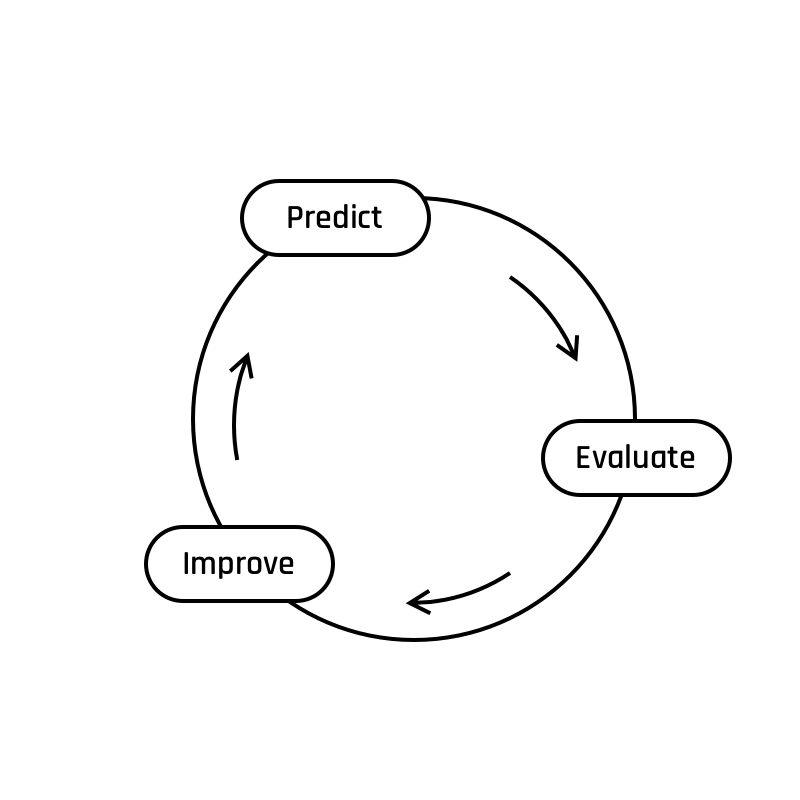
\includegraphics[scale=0.25]{assets/Default.png}
    %\caption{The Learning Cycle}
\end{figure}
\\
The first algorithm you discovered, \textbf{Multivariate Linear Regression}, can now be used to predict a numerical value, based on several features.
This algorithm uses gradient descent to optimize its loss function.\\
\\
Now let's introduce your first \textbf{classification algorithm}: the notorious \textbf{Logistic Regression.}
\hint{regression vs classification; discrete vs continuous values}
\newpage
\noindent{\textbf{Logistic regression} performs a \textit{classification task}, which means that you are not predicting a numerical value (like price, age, grades...) 
but \textbf{categories}, or \textbf{labels} (like dog, cat, sick/healty...)}.
\\
\warn{
    Don't be confused by the word \textit{'regression'} in \textbf{Logistic Regression}.
    It really is a \textit{classification task}! The name is a bit tricky but you will quickly get used to it.
    Once again: \textbf{Logistic Regression is a classification algorithm} which assigns a label/category/class to a given example.
}
\info{
    In this module we will use the following terms interchangeably: \textbf{class}, \textbf{category}, and \textbf{label}.
    They all refer to the \textit{groups} to which each training example can be assigned to, in a classification task.
}

% =============================== %
\subsection*{Predict I: Introducing the Sigmoid Function}
% ******************************* %

\begin{figure}[!h]
    \centering
    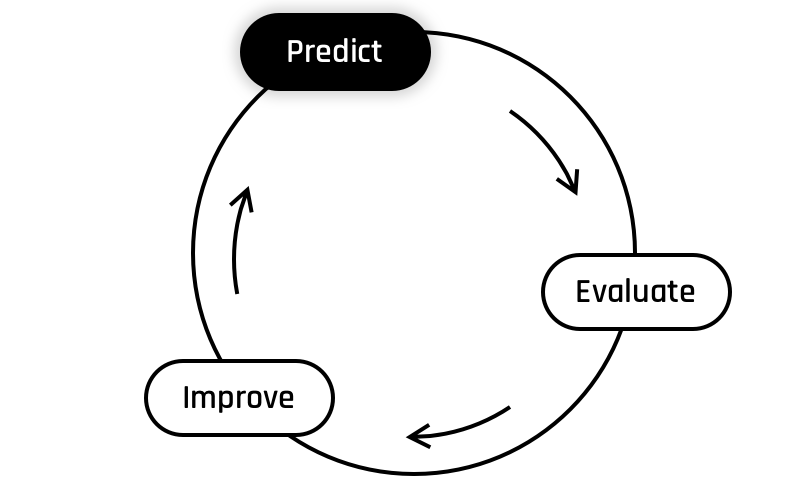
\includegraphics[scale=0.25]{assets/Predict.png}
    %\caption{The Learning Cycle - Predict}
\end{figure}

% =============================== %
\subsubsection*{Formulating a Hypothesis}
% ******************************* %
Remember that a hypothesis, denoted $h(\theta)$, is an equation that combines a set of \textbf{features} (that characterizes an example) with \textbf{parameters} in order to output a \textbf{prediction}.\\
\\
Remember the hypothesis we used in linear regression?\\
$$
h(\theta) = \theta_0 + \theta_{1} x_{1}^{(i)} + \dots + \theta_{n} x_{n}^{(i)} = \theta \cdot x'^{(i)}
$$
\newline
It worked fine to predict continuous values, but could we also use it to tell, for example, 
if a patient is sick or not?
That's a yes-or-no question, so the output from the hypothesis function should reflect that.\\
\\
To get started, we will assign each class a numerical value: sick patients will be 
assigned a value of 1, and healthy patients will be assigned a value of 0.\\
The goal will be to build a hypothesis that outputs a probability that a patient is sick as a float number in the range of [0, 1].\\
\\
The good news is that we can keep the linear equation we already worked with!\\
\\
All we need to do is squash its output through another function that is bounded between 0 and 1.\\
\\
That's the purpose of the \textbf{Sigmoid function} and your next assignment is to implement it!

%\newpage
\turnindir{ex00}
\exnumber{00}
\exfiles{polynomial\_model\_extended.py}
\exforbidden{sklearn}
\makeheaderfilesforbidden

% ================================== %
\section*{Objective}
% ---------------------------------- %
Create a function that takes a matrix $X$ of dimensions $(m \times n)$ and an integer $p$ as input, and returns a matrix of dimension $(m \times (np))$.
For each column $x_j$ of the matrix $X$, the new matrix contains
$x_j$ raised to the power of $k$, for $k = 1, 2, ..., p$ :

$$
x_1  \mid  \ldots  \mid  x_n  \mid  x_1^2  \mid  \ldots  \mid  x_n^2  \mid  \ldots  \mid  x_1^p  \mid  \ldots  \mid  x_n^p
$$

% ================================== %
\section*{Instructions}
% ---------------------------------- %
In the \texttt{polynomial\_model\_extended.py} file, write the following function as per the instructions given below:

\begin{minted}[bgcolor=darcula-back,formatcom=\color{lightgrey},fontsize=\scriptsize]{python}
def add_polynomial_features(x, power):
	"""Add polynomial features to matrix x by raising its columns to every power in the range of 1 up to the power given in argument.  
	Args:
		x: has to be an numpy.ndarray, a matrix of shape m * n.
		power: has to be an int, the power up to which the columns of matrix x are going to be raised.
	Returns:
		The matrix of polynomial features as a numpy.ndarray, of shape m * (np), containg the polynomial feature values for all training examples.
		None if x is an empty numpy.ndarray.
	Raises:
		This function should not raise any Exception.
	"""
	... Your code ...
\end{minted}


% ================================== %
\section*{Examples}
% ---------------------------------- %

\begin{minted}[bgcolor=darcula-back,formatcom=\color{lightgrey},fontsize=\scriptsize]{python}
import numpy as np
x = np.arange(1,11).reshape(5, 2)

# Example 1:
add_polynomial_features(x, 3)
# Output:
array([[   1,    2,    1,    4,    1,    8],
       [   3,    4,    9,   16,   27,   64],
       [   5,    6,   25,   36,  125,  216],
       [   7,    8,   49,   64,  343,  512],
       [   9,   10,   81,  100,  729, 1000]])

# Example 2:
add_polynomial_features(x, 4)
# Output:
array([[    1,     2,     1,     4,     1,     8,     1,    16],
       [    3,     4,     9,    16,    27,    64,    81,   256],
       [    5,     6,    25,    36,   125,   216,   625,  1296],
       [    7,     8,    49,    64,   343,   512,  2401,  4096],
       [    9,    10,    81,   100,   729,  1000,  6561, 10000]])
\end{minted}

% ===========================(fin ex 00)         %
% ============================================== %

\newpage

% ============================================== %
% ===========================(start ex 01)       %
\chapter{Exercise 01}
\extitle{L2 Regularization}
%******************************************************************************%
%                                                                              %
%                                 Interlude                                    %
%                         for Machine Learning module                          %
%                                                                              %
%******************************************************************************%

% =============================== %
\section*{Linear Algebra Tricks part II}
% ******************************* %

If you tried to run your code on a very large dataset, you would find that it sometimes takes a (very) long time to execute!
That's because it doesn't use the power of Python libraries that are optimized for matrix operations.\\
\newline
Remember the linear algebra trick from the previous module? Let's use it again!  
If you concatenate a column of $1$'s to the left of the $x$ vector, you get what we called matrix $X'$.   
$$
X' = \begin{bmatrix} 1 & x^{(1)} \\ \vdots & \vdots \\ 1 & x^{(m)}\end{bmatrix}
$$
This transformation is very convenient because we can rewrite each $1$ as $x_0^{(i)}$, and each $x^{(i)}$ as $x_1^{(i)}$.
So now the $X'$ matrix looks like this:
$$
X' = \begin{bmatrix} x_0^{(1)} & x_1^{(1)} \\ \vdots & \vdots \\ x_0^{(m)} & x_1^{(m)}\end{bmatrix}
$$
Notice that each $x^{(i)}$ example becomes a vector made of $(x^{(i)}_0, x^{(i)}_1)$.  
The $0$ and $1$ indices on the $x$ features correspond to the indices of the $\theta$ parameters with which they will be multiplied.\\
\newline
Why does this matter?
Well, if we take the equation from the previous exercise:

$$
\nabla(J)_0 = \frac{1}{m}\sum_{i=1}^{m}(h_{\theta}(x^{(i)}) - y^{(i)})
$$
We can multiply it by $1$ without changing its value:
$$
\nabla(J)_0 = \frac{1}{m}\sum_{i=1}^{m}(h_{\theta}(x^{(i)}) - y^{(i)}) \cdot 1
$$
And rewrite $1$ as $x_0^{(i)}$:
$$
\nabla(J)_0 = \frac{1}{m}\sum_{i=1}^{m}(h_{\theta}(x^{(i)}) - y^{(i)})x_{0}^{(i)}
$$
This means that the equation for $\nabla(J)_0$ is now similar to the equation we had for $\nabla(J)_1$, so they can both be captured by ONE \textbf{generic equation}:
$$
\begin{matrix}
\nabla(J)_j = \frac{1}{m}\sum_{i=1}^{m}(h_{\theta}(x^{(i)}) - y^{(i)})x_{j}^{(i)} & & \text{ for j = 0, 1}    
\end{matrix}
$$
And as you probably suspected, a generic equation opens the door to vectorization...

% =============================== %
\subsection*{Vectorizing the Gradient Calculation}
% ******************************* %
Now it's time to learn how to calculate the entire gradient in one short, pretty, linear algebra equation!  
\begin{itemize}
    \item First, we'll use the $X'$ matrix and our vectorized hypothesis equation $h_{\theta}(x)=X'\theta$
    $$
    \begin{matrix}
    \nabla(J)_j = \frac{1}{m} (X'\theta - y)X'_{j} & & \text{ for j = 0, 1}
    \end{matrix}
    $$
    
    \item Second, we need to tweak the equation a bit so that it directly returns a $\nabla(J)$ vector containing both $\nabla(J)_0$ and $\nabla(J)_1$.
    
    $$
    \nabla(J) = \frac{1}{m} {X'}^T(X'\theta - y)    
    $$
\end{itemize}
If the equation does not seems obvious, play a bit with your vectors, on paper and in your code, until you get it.\\

% =============================== %
\subsubsection*{Notation Remark}
% ******************************* %
${X'}^T$: You might wonder what the $^T$ is for.
It means the $X'$ matrix must be \textbf{transposed}.\\
\newline
Transposing a matrix flips it on its diagonal so that its rows become its columns and \textit{vice-versa}.
Here we need to make sure that matrix dimensions are appropriate and allow for multiplication, and to multiply the right items together.
\newpage
\turnindir{ex01}
\exnumber{01}
\exfiles{l2\_reg.py}
\exforbidden{sklearn}
\makeheaderfilesforbidden

% ================================= %
\section*{Objective}
% --------------------------------- %
You must implement the following formulas as functions:  

% ================================= %
\subsection*{Iterative}
% --------------------------------- %
$$
L_2(\theta)^2 = \sum_{j = 1}^n \theta_j^2
$$

Where:
\begin{itemize}
  \item $\theta$ is a vector of dimension $(n + 1)$.
\end{itemize}

% ================================= %
\subsection*{Vectorized}
% --------------------------------- %
$$
L_2(\theta)^2 = \theta' \cdot \theta'
$$

Where:
\begin{itemize}
  \item $\theta'$ is a vector of dimension $(n + 1)$, constructed using the following rules:
\end{itemize}
  
$$
\begin{matrix}
\theta'_0 & =  0 \\
\theta'_j & =  \theta_j & \text{ for } j = 1, \dots, n\\
\end{matrix}
$$

% ================================= %
\section*{Instructions}
% --------------------------------- %
In the \texttt{l2\_reg.py} file, write the following function as per the instructions given below:

\begin{minted}[bgcolor=darcula-back,formatcom=\color{lightgrey},fontsize=\scriptsize]{python}
def iterative_l2(theta):
	"""Computes the L2 regularization of a non-empty numpy.ndarray, with a for-loop.
	Args:
		theta: has to be a numpy.ndarray, a vector of shape n * 1.
	Returns:
		The L2 regularization as a float.
		None if theta in an empty numpy.ndarray.
	Raises:
		This function should not raise any Exception.
	"""
	... Your code ...

def l2(theta):
	"""Computes the L2 regularization of a non-empty numpy.ndarray, without any for-loop.
	Args:
		theta: has to be a numpy.ndarray, a vector of shape n * 1.
	Returns:
		The L2 regularization as a float.
		None if theta in an empty numpy.ndarray.
	Raises:
		This function should not raise any Exception.
	"""
	... Your code ...
\end{minted}

% ================================= %
\section*{Examples}
% --------------------------------- %

\begin{minted}[bgcolor=darcula-back,formatcom=\color{lightgrey},fontsize=\scriptsize]{python}
x = np.array([2, 14, -13, 5, 12, 4, -19]).reshape((-1, 1))

# Example 1: 
iterative_l2(x)
# Output:
911.0

# Example 2: 
l2(x)
# Output:
911.0

y = np.array([3,0.5,-6]).reshape((-1, 1))
# Example 3: 
iterative_l2(y)
# Output:
36.25

# Example 4: 
l2(y)
# Output:
36.25
\end{minted}

% ===========================(fin ex 01)         %
% ============================================== %

\newpage

% ============================================== %
% ===========================(start ex 02)       %
\chapter{Exercise 02}
\extitle{Regularized Linear Loss Function}

\turnindir{ex02}
\exnumber{02}
\exfiles{linear\_loss\_reg.py}
\exforbidden{sklearn}
\makeheaderfilesforbidden

% ================================= %
\section*{Objective}
% --------------------------------- %
You must implement the following formula as a function:  

$$
J(\theta)  =  \frac{1}{2m}[(\hat{y} - y)\cdot(\hat{y} - y) + \lambda (\theta' \cdot \theta')]
$$  

Where:
\begin{itemize}
  \item $y$ is a vector of dimension $m$, the expected values,
  \item $\hat{y}$ is a vector of dimension $m$, the predicted values,
  \item $\lambda$ is a constant, the regularization hyperparameter,
  \item $\theta'$ is a vector of dimension $n$, constructed using the following rules:
\end{itemize}
  
$$
\begin{matrix}
\theta'_0 & =  0 \\
\theta'_j & =  \theta_j & \text{ for } j = 1, \dots, n\\
\end{matrix}
$$

% ================================= %
\section*{Instructions}
% --------------------------------- %
In the \texttt{linear\_loss\_reg.py} file, write the following function as per the instructions given below:

\begin{minted}[bgcolor=darcula-back,formatcom=\color{lightgrey},fontsize=\scriptsize]{python}
def reg_loss_(y, y_hat, theta, lambda_):
	"""Computes the regularized loss of a linear regression model from two non-empty numpy.array, without any for loop. The two arrays must have the same dimensions.
	Args:
		y: has to be an numpy.ndarray, a vector of shape m * 1.
		y_hat: has to be an numpy.ndarray, a vector of shape m * 1.
		theta: has to be a numpy.ndarray, a vector of shape n * 1.
		lambda_: has to be a float.
	Returns:
		The regularized loss as a float.
		None if y, y_hat, or theta are empty numpy.ndarray.
		None if y and y_hat do not share the same shapes.
	Raises:
		This function should not raise any Exception.
	"""
	... Your code ...
\end{minted}

\hint{such situation is a good use case for decorators...}

% ================================= %
\section*{Examples}
% --------------------------------- %
\begin{minted}[bgcolor=darcula-back,formatcom=\color{lightgrey},fontsize=\scriptsize]{python}
y = np.array([2, 14, -13, 5, 12, 4, -19]).reshape((-1, 1))
y_hat = np.array([3, 13, -11.5, 5, 11, 5, -20]).reshape((-1, 1))
theta = np.array([1, 2.5, 1.5, -0.9]).reshape((-1, 1))

# Example :
reg_loss_(y, y_hat, theta, .5)
# Output:
0.8503571428571429

# Example :
reg_loss_(y, y_hat, theta, .05)
# Output:
0.5511071428571429

# Example :
reg_loss_(y, y_hat, theta, .9)
# Output:
1.116357142857143
\end{minted}


% ===========================(fin ex 02)         %
% ============================================== %

\newpage

% ============================================== %
% ===========================(start ex 03)       %
\chapter{Exercise 03}
\extitle{Regularized Logistic Loss Function}
%%******************************************************************************%
%                                                                              %
%                                 Interlude                                    %
%                         for Machine Learning module                          %
%                                                                              %
%******************************************************************************%

% =============================== %
\section*{Interlude}
% =============================== %
\subsection*{Linear Algebra Strikes Again!}
% ******************************* %

You've become quite used to vectorization by now.
You may have already tried to vectorize the logistic loss function by yourself.
Let's look one last time at the former equation:

$$
J( \theta) = -\cfrac{1} {m} \lbrack \sum_{i = 1}^{m} y^{(i)}\log(\hat{y}^{(i)})) + (1 - y^{(i)})\log(1 - \hat{y}^{(i)})\rbrack
$$

% =============================== %
\subsection*{Vectorized Logistic Loss Function}
% ******************************* %
In the \textbf{vectorized version}, we remove the sum ($\sum$) because it is captured by the dot products:
$$
J( \theta) = -\cfrac{1} {m} \lbrack y \cdot \log(\hat{y}) + (\vec{1} - y) \cdot \log(\vec{1} - \hat{y})\rbrack
$$

Where:
\begin{itemize}
       \item $\vec{1}$ is a vector full of $1$'s with the same dimension of $y$ ($m$).
             $$
             \vec{1} = \begin{bmatrix}
                 1 \\
                 \vdots \\
                 1
             \end{bmatrix}
             $$
\end{itemize}


% =============================== %
\subsection*{Note: Operations Between Vectors and Scalars}
% ******************************* %
We use the $\vec{1}$ notation to be rigorous, because \textbf{addition (or subtraction) between a vector and a scalar is not defined}.
In other words, mathematically, you cannot write this: $1 - y$.
The only operation defined between a scalar and a vector is multiplication, remember?

% =============================== %
\subsubsection*{However...}
% ******************************* %
\texttt{NumPy} is a bit permissive on vectors and matrix operations...
The following instructions will get you the same results:

\begin{minted}[bgcolor=darcula-back,formatcom=\color{lightgrey},fontsize=\scriptsize]{python}
# Proper mathematical notation
y = np.array([[4], [7.16], [3.2], [9.37], [0.56]])
ones = np.ones(y.shape[0]).reshape((-1,1))
ones - y
# Output
array([[-3.  ],
       [-6.16],
       [-2.2 ],
       [-8.37],
       [ 0.44]])

# Incorrect mathematical notation
y = np.array([[4], [7.16], [3.2], [9.37], [0.56]])
1 - y
# Output
array([[-3.  ],
       [-6.16],
       [-2.2 ],
       [-8.37],
       [ 0.44]])
\end{minted}

Strange, isn't it?
It happens because of one of \texttt{NumPy}'s permissive operations called \textbf{Broadcasting}.
Broadcasting is a powerful feature whereby \texttt{NumPy} is able to figure out that you actually wanted to perform a subtraction on each element in the vector, so it does it for you automatically.
It's very handy to write concise lines of code, but it can insert very sneaky bugs if you aren't $100$\% confident in what you're doing.


Many of the bugs you will encounter while working on Machine Learning problems will come from \texttt{NumPy}'s permissiveness.
Such bugs generaly don't throw any errors, but mess up the content of your vectors and matrices and you'll spend an awful lot of time looking for why your model doesn't learn.
This is why we \textbf{strongly} suggest that you pay attention to your vector (and matrix) shapes and \textbf{stick as much as possible to the actual mathematical operations}.

For more information, you can watch \href{https://www.youtube.com/watch?v=V2QlTmh6P2Y&t=213s}{this video on dealing with Broadcasting}.

%\newpage
\turnindir{ex03}
\exnumber{03}
\exfiles{logistic\_loss\_reg.py}
\exforbidden{sklearn}
\makeheaderfilesforbidden

% ================================= %
\section*{Objective}
% --------------------------------- %
You must implement the following formula as a function:

$$
J( \theta) = -\frac{1} {m} \lbrack y \cdot \log(\hat{y}) + (\vec{1} - y) \cdot \log(\vec{1} - \hat{y})\rbrack + \frac{\lambda}{2m} (\theta' \cdot \theta')
$$

Where:
\begin{itemize}
  \item $\hat{y}$ is a vector of dimension $m$, the vector of predicted values,
  \item $y$ is a vector of dimension $m$, the vector of expected values,
  \item $\vec{1}$ is a vector of dimension $m$, a vector full of ones,
  \item $\lambda$ is a constant, the regularization hyperparameter,
  \item $\theta'$ is a vector of dimension $n$, constructed using the following rules: 
\end{itemize}
$$
\begin{matrix}
\theta'_0 & =  0 \\
\theta'_j & =  \theta_j & \text{ for } j = 1, \dots, n\\    
\end{matrix}
$$

% ================================= %
\section*{Instructions}
% --------------------------------- %
In the \texttt{logistic\_loss\_reg.py} file, write the following function as per the instructions given below:

\begin{minted}[bgcolor=darcula-back,formatcom=\color{lightgrey},fontsize=\scriptsize]{python}
def reg_log_loss_(y, y_hat, theta, lambda_):
	"""Computes the regularized loss of a logistic regression model from two non-empty numpy.ndarray, without any for loop. The two arrays must have the same shapes.
	Args:
		y: has to be an numpy.ndarray, a vector of shape m * 1.
		y_hat: has to be an numpy.ndarray, a vector of shape m * 1.
		theta: has to be a numpy.ndarray, a vector of shape n * 1.
		lambda_: has to be a float.
	Returns:
		The regularized loss as a float.
		None if y, y_hat, or theta is empty numpy.ndarray.
		None if y and y_hat do not share the same shapes.
	Raises:
		This function should not raise any Exception.
	"""
	... Your code ...
\end{minted}

\hint{
  this is a good use case for decorators...
}


% ================================= %
\section*{Examples}
% --------------------------------- %
\begin{minted}[bgcolor=darcula-back,formatcom=\color{lightgrey},fontsize=\scriptsize]{python}
y = np.array([1, 1, 0, 0, 1, 1, 0]).reshape((-1, 1))
y_hat = np.array([.9, .79, .12, .04, .89, .93, .01]).reshape((-1, 1))
theta = np.array([1, 2.5, 1.5, -0.9]).reshape((-1, 1))

# Example :
reg_log_loss_(y, y_hat, theta, .5)
# Output:
0.43377043716475955

# Example :
reg_log_loss_(y, y_hat, theta, .05)
# Output:
0.13452043716475953

# Example :
reg_log_loss_(y, y_hat, theta, .9)
# Output:
0.6997704371647596
\end{minted}

% ===========================(fin ex 03)         %
% ============================================== %

\newpage

% ============================================== %
% ===========================(start ex 04)       %
\chapter{Exercise 04}
\extitle{Regularized Linear Gradient}
%******************************************************************************%
%                                                                              %
%                                 Interlude                                    %
%                         for Machine Learning module                          %
%                                                                              %
%******************************************************************************%

% =============================================== %
\section*{Interlude - Regularized Gradient}
% =============================================== %
\begin{figure}[!h]
    \centering
    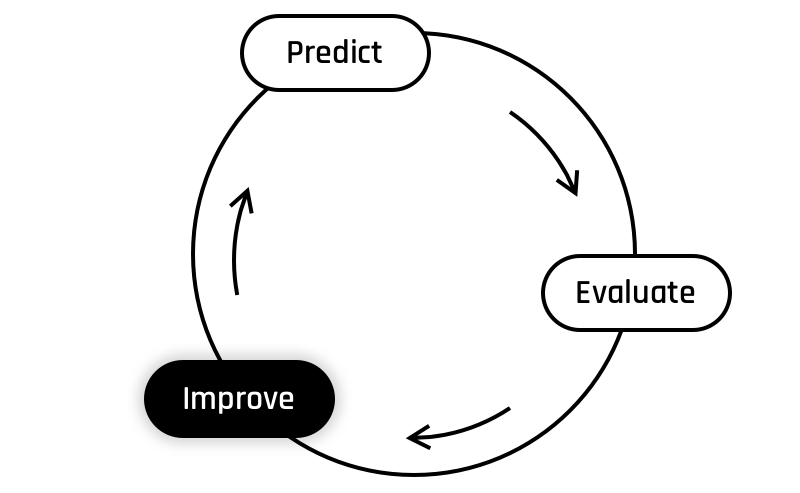
\includegraphics[scale=0.25]{assets/Improve.png}
    %\caption{The Learning Cycle: Improve}
\end{figure}
\noindent{To derive the gradient of the regularized loss function, $\nabla(J)$ 
you have to change a bit the formula of the unregularized gradient.}\\
\\
Given the fact that we are not penalizing $\theta_0$, the formula will remain 
the same as before for this parameter. For the other parameters ($\theta_1, \dots, \theta_n$),
 we must add the partial derivative of the regularization term: $\lambda \theta_j$.\\
\\
Therefore, we get:
$$
\nabla(J)_0 = \frac{1}{m}\sum_{i=1}^{m}(h_\theta(x^{(i)}) - y^{(i)})
$$
$$
\nabla(J)_j = \frac{1}{m}\left(\sum_{i=1}^{m}(h_\theta(x^{(i)}) - y^{(i)})x_j^{(i)} + \lambda \theta_j\right) \text{ for j = 1, ..., n}
$$
\\
Where:  
\begin{itemize}
    \item $\nabla(J)_j$ is the j$^\text{th}$ component of the gradient vector $\nabla(J)$
    \item $m$ is the number of training examples used
    \item $h_\theta(x^{(i)})$ is the model's prediction for the i$^\text{th}$ training example
    \item $x^{(i)}$ is the feature vector of the i$^\text{th}$ training example
    \item $y^{(i)}$ is the expected target value for the i$^\text{th}$ example
    \item $\lambda$ is a constant, the regularization hyperparameter
    \item $\theta_j$ is the j$^\text{th}$ parameter of the $\theta$ vector
\end{itemize}
\bigskip
Which can be vectorized as:
$$
\nabla(J) = \frac{1}{m} [X'^T(h_\theta(X) - y) + \lambda \theta']
$$  
\\
Where:  
\begin{itemize}
    \item $\nabla(J)$ is a vector of length $(n + 1)$, the gradient vector
    \item $m$ is the number of training examples used
    \item $X$ is a matrix of dimension $(m \times n)$, the design matrix
    \item $X'$ is a matrix of dimension $(m \times (n + 1))$, the design matrix onto 
    which a column of ones is added as a first column
    \item $y$ is a vector of length $m$, the vector of expected values
    \item $h_\theta(X)$ is a vector of length $m$, the vector of predicted values
    \item $\lambda$ is a constant
    \item $\theta$ is a vector of length $(n + 1)$, the parameter vector
    \item $\theta'$ is a vector of length $(n + 1)$, constructed using the following rules:
\end{itemize}

$$
\begin{matrix}
\theta'_0 & =  0 \\
\theta'_j & =  \theta_j & \text{ for } j = 1, \dots, n\\    
\end{matrix}
$$

% =============================================== %
\subsection*{Linear Gradient vs Logistic Gradient}
% ----------------------------------------------- %
As before, we draw your attention on the only difference between the linear regression's 
and the logistic regression's gradient equations: \textbf{the hypothesis function} $h_\theta(X)$.
\begin{itemize}
    \item In the linear regression: $h_\theta(X) = X'\theta$
    \item In the logistic regression: $h_\theta(X) = \text{sigmoid}(X'\theta)$
\end{itemize}

\newpage
\turnindir{ex04}
\exnumber{04}
\exfiles{reg\_linear\_grad.py}
\exforbidden{sklearn}
\makeheaderfilesforbidden


% ================================= %
\section*{Objective}
% --------------------------------- %
You must implement the following formulas as a functions for the \textbf{linear regression hypothesis}:

% ================================= %
\subsection*{Iterative}
% --------------------------------- %
$$
\nabla(J)_0 = \frac{1}{m}\sum_{i=1}^{m}(h_\theta(x^{(i)}) - y^{(i)})
$$
$$
\nabla(J)_j = \frac{1}{m}\left(\sum_{i=1}^{m}(h_\theta(x^{(i)}) - y^{(i)})x_j^{(i)} + \lambda \theta_j\right) \text{ for j = 1, ..., n}
$$

Where:
\begin{itemize}
  \item $\nabla(J)_j$ is the j$^\text{th}$ component of $\nabla(J)$,
  \item $\nabla(J)$ is a vector of dimension $(n + 1)$, the gradient vector,
  \item $m$ is a constant, the number of training examples used,
  \item $h_\theta(x^{(i)})$ is the model's prediction for the i$^\text{th}$ training example,
  \item $x^{(i)}$ is the feature vector (of dimension $n$) of the i$^\text{th}$ training example, found in the i$^\text{th}$ row of the $X$ matrix,
  \item $X$ is a matrix of dimensions $(m \times n)$, the design matrix,
  \item $y^{(i)}$ is the i$^\text{th}$ component of the $y$ vector,
  \item $y$ is a vector of dimension $m$, the vector of expected values,
  \item $\lambda$ is a constant, the regularization hyperparameter,
  \item $\theta_j$ is the j$^\text{th}$ parameter of the $\theta$ vector,
  \item $\theta$ is a vector of dimension $(n + 1)$, the parameter vector.
\end{itemize}

% ================================= %
\subsection*{Vectorized}
% --------------------------------- %
$$
\nabla(J) = \frac{1}{m} [X'^T(h_\theta(X) - y) + \lambda \theta']
$$  

Where:
\begin{itemize}
  \item $\nabla(J)$ is a vector of dimension $(n + 1)$, the gradient vector,
  \item $m$ is a constant, the number of training examples used,
  \item $X$ is a matrix of dimensions $(m \times n)$, the design matrix,
  \item $X'$ is a matrix of dimensions $(m \times (n + 1))$, the design matrix onto which a column of ones is added as a first column,
  \item $X'^T$ is the transpose of tha matrix, with dimensions $((n + 1) \times m)$,
  \item $h_\theta(X)$ is a vector of dimension $m$, the vector of predicted values, 
  \item $y$ is a vector of dimension $m$, the vector of expected values,
  \item $\lambda$ is a constant, the regularization hyperparameter,
  \item $\theta$ is a vector of dimension $(n + 1)$, the parameter vector,
  \item $\theta'$ is a vector of dimension $(n + 1)$, constructed using the following rules: 
\end{itemize}

$$
\begin{matrix}
\theta'_0 & =  0 \\
\theta'_j & =  \theta_j & \text{ for } j = 1, \dots, n\\
\end{matrix}
$$

% ================================= %
\section*{Instructions}
% --------------------------------- %
In the \texttt{reg\_linear\_grad.py} file, write the following functions as per the instructions given below:

\begin{minted}[bgcolor=darcula-back,formatcom=\color{lightgrey},fontsize=\scriptsize]{python}
def reg_linear_grad(y, x, theta, lambda_):
    """Computes the regularized linear gradient of three non-empty numpy.ndarray,
       with two for-loop. The three arrays must have compatible shapes.
    Args:
      y: has to be a numpy.ndarray, a vector of shape m * 1.
      x: has to be a numpy.ndarray, a matrix of dimesion m * n.
      theta: has to be a numpy.ndarray, a vector of shape (n + 1) * 1.
      lambda_: has to be a float.
    Return:
      A numpy.ndarray, a vector of shape (n + 1) * 1, containing the results of the formula for all j.
      None if y, x, or theta are empty numpy.ndarray.
      None if y, x or theta does not share compatibles shapes.
      None if y, x or theta or lambda_ is not of the expected type.
    Raises:
      This function should not raise any Exception.
    """
    ... Your code ...

def vec_reg_linear_grad(y, x, theta, lambda_):
    """Computes the regularized linear gradient of three non-empty numpy.ndarray,
       without any for-loop. The three arrays must have compatible shapes.
    Args:
      y: has to be a numpy.ndarray, a vector of shape m * 1.
      x: has to be a numpy.ndarray, a matrix of dimesion m * n.
      theta: has to be a numpy.ndarray, a vector of shape (n + 1) * 1.
      lambda_: has to be a float.
    Return:
      A numpy.ndarray, a vector of shape (n + 1) * 1, containing the results of the formula for all j.
      None if y, x, or theta are empty numpy.ndarray.
      None if y, x or theta does not share compatibles shapes.
      None if y, x or theta or lambda_ is not of the expected type.
    Raises:
      This function should not raise any Exception.
    """
    ... Your code ...
\end{minted}

\hint{
  this is a good use case for decorators...
}

% ================================= %
\section*{Examples}
% ================================= %
\begin{minted}[bgcolor=darcula-back,formatcom=\color{lightgrey},fontsize=\scriptsize]{python}
x = np.array([
		[ -6,  -7,  -9],
		[ 13,  -2,  14],
		[ -7,  14,  -1],
		[ -8,  -4,   6],
		[ -5,  -9,   6],
		[  1,  -5,  11],
		[  9, -11,   8]])
y = np.array([[2], [14], [-13], [5], [12], [4], [-19]])
theta = np.array([[7.01], [3], [10.5], [-6]])

# Example 1.1:
reg_linear_grad(y, x, theta, 1)
# Output:
array([[ -60.99      ],
		[-195.64714286],
		[ 863.46571429],
		[-644.52142857]])

# Example 1.2:
vec_reg_linear_grad(y, x, theta, 1)
# Output:
array([[ -60.99      ],
		[-195.64714286],
		[ 863.46571429],
		[-644.52142857]])

# Example 2.1:
reg_linear_grad(y, x, theta, 0.5)
# Output:
array([[ -60.99      ],
		[-195.86142857],
		[ 862.71571429],
		[-644.09285714]])

# Example 2.2:
vec_reg_linear_grad(y, x, theta, 0.5)
# Output:
array([[ -60.99      ],
		[-195.86142857],
		[ 862.71571429],
		[-644.09285714]])

# Example 3.1:
reg_linear_grad(y, x, theta, 0.0)
# Output:
array([[ -60.99      ],
		[-196.07571429],
		[ 861.96571429],
		[-643.66428571]])

# Example 3.2:
vec_reg_linear_grad(y, x, theta, 0.0)
# Output:
array([[ -60.99      ],
		[-196.07571429],
		[ 861.96571429],
		[-643.66428571]])
\end{minted}


% ===========================(fin ex 04)         %
% ============================================== %

\newpage

% ============================================== %
% ===========================(start ex 05)       %
\chapter{Exercise 05}
\extitle{Regularized Logistic Gradient}
%%******************************************************************************%
%                                                                              %
%                                 Interlude                                    %
%                         for Machine Learning module                          %
%                                                                              %
%******************************************************************************%

\section*{Interlude - Normalization}

The values inside the $x$ vector can vary quite a lot in magnitude,
depending on the type of data you are working with.
For example, if your dataset contains distances between planets in km, the numbers will be huge.
On the other hand, if you are working with planet masses expressed as a fraction of the solar system's total mass, the numbers will be very small (between 0 and 1).
Both cases may slow down convergence in Gradient Descent (or even sometimes prevent convergence at all).
To avoid that kind of situation, normalization is a very effective way to proceed.


The idea behind this technique is straightforward: \textbf{scaling the data}.  


With normalization, you can transform your $x$ vector into a new $x'$ vector whose values range between $[-1, 1]$ more or less. Doing this allows you to see much more easily how a training example compares to the other ones:
\begin{itemize}
    \item If an $x'$ value is close to $1$, you know it's among the largest in the dataset
    \item If an $x'$ value is close to $0$, you know it's close to the median
    \item If an $x'$ value is close to $-1$, you know it's among the smallest
\end{itemize}

So with the upcoming normalization techniques, you'll be able to map your data to two different value ranges: $[0, 1]$ or $[-1, 1]$. Your algorithm will like it and thank you for it.  

%\newpage
\turnindir{ex05}
\exnumber{05}
\exfiles{reg\_logistic\_grad.py}
\exforbidden{sklearn}
\makeheaderfilesforbidden

% ================================= %
\section*{Objective}
% --------------------------------- %
You must implement the following formulas as a functions for the \textbf{logistic regression hypothesis}:

% ================================= %
\subsection*{Iterative}
% --------------------------------- %

$$
\nabla(J)_0 = \frac{1}{m}\sum_{i=1}^{m}(h_\theta(x^{(i)}) - y^{(i)})
$$
$$
\nabla(J)_j = \frac{1}{m}\left(\sum_{i=1}^{m}(h_\theta(x^{(i)}) - y^{(i)})x_j^{(i)} + \lambda \theta_j\right) \text{ for j = 1, ..., n}
$$

Where:
\begin{itemize}
  \item $\nabla(J)_j$ is the j$^\text{th}$ component of $\nabla(J)$,
  \item $\nabla(J)$ is a vector of dimension $(n + 1)$, the gradient vector,
  \item $m$ is a constant, the number of training examples used,
  \item $h_\theta(x^{(i)})$ is the model's prediction for the i$^\text{th}$ training example,
  \item $x^{(i)}$ is the feature vector of dimension $n$) of the i$^\text{th}$ training example, found in the i$^\text{th}$ row of the $X$ matrix,
  \item $X$ is a matrix of dimensions $(m \times n)$, the design matrix,
  \item $y^{(i)}$ is the i$^\text{th}$ component of the $y$ vector,
  \item $y$ is a vector of dimension $m$, the vector of expected values,
  \item $\lambda$ is a constant, the regularization hyperparameter,
  \item $\theta_j$ is the j$^\text{th}$ parameter of the $\theta$ vector,
  \item $\theta$ is a vector of dimension $(n + 1)$, the parameter vector.
\end{itemize}

% ================================= %
\subsection*{Vectorized}
% --------------------------------- %
$$
\nabla(J) = \frac{1}{m} [X'^T(h_\theta(X) - y) + \lambda \theta']
$$  

Where:
\begin{itemize}
  \item $\nabla(J)$ is a vector of dimension $(n + 1)$, the gradient vector,
  \item $m$ is a constant, the number of training examples used,
  \item $X$ is a matrix of dimensions $(m \times n)$, the design matrix,
  \item $X'$ is a matrix of dimensions $(m \times (n + 1))$, the design matrix onto which a column of ones is added as a first column,
  \item $X'^T$ is the transpose of tha matrix, with dimensions $((n + 1) \times m)$,
  \item $h_\theta(X)$ is a vector of dimension $m$, the vector of predicted values, 
  \item $y$ is a vector of dimension $m$, the vector of expected values,
  \item $\lambda$ is a constant, the regularization hyperparameter,
  \item $\theta$ is a vector of dimension $(n + 1)$, the parameter vector,
  \item $\theta'$ is a vector of dimension $(n + 1)$, constructed using the following rules: 
\end{itemize}

$$
\begin{matrix}
\theta'_0 & =  0 \\
\theta'_j & =  \theta_j & \text{ for } j = 1, \dots, n\\
\end{matrix}
$$

% ================================= %
\section*{Instructions}
% --------------------------------- %
In the \texttt{reg\_logistic\_grad.py} file, create the following function as per the instructions given below:

\begin{minted}[bgcolor=darcula-back,formatcom=\color{lightgrey},fontsize=\scriptsize]{python}
def reg_logistic_grad(y, x, theta, lambda_):
	"""Computes the regularized logistic gradient of three non-empty numpy.ndarray, with two for-loops. The three arrays must have compatible shapes.
	Args:
		y: has to be a numpy.ndarray, a vector of shape m * 1.
		x: has to be a numpy.ndarray, a matrix of dimesion m * n.
		theta: has to be a numpy.ndarray, a vector of shape n * 1.
		lambda_: has to be a float.
	Returns:
		A numpy.ndarray, a vector of shape n * 1, containing the results of the formula for all j.
		None if y, x, or theta are empty numpy.ndarray.
		None if y, x or theta does not share compatibles shapes.
	Raises:
		This function should not raise any Exception.
	"""
	... Your code ...

def vec_reg_logistic_grad(y, x, theta, lambda_):
	"""Computes the regularized logistic gradient of three non-empty numpy.ndarray, without any for-loop. The three arrays must have compatible shapes.
	Args:
		y: has to be a numpy.ndarray, a vector of shape m * 1.
		x: has to be a numpy.ndarray, a matrix of shape m * n.
		theta: has to be a numpy.ndarray, a vector of shape n * 1.
		lambda_: has to be a float.
	Returns:
		A numpy.ndarray, a vector of shape n * 1, containing the results of the formula for all j.
		None if y, x, or theta are empty numpy.ndarray.
		None if y, x or theta does not share compatibles shapes.
	Raises:
		This function should not raise any Exception.
	"""
	... Your code ...
\end{minted}

\hint{
  this is a good use case for decorators...
}

% ================================= %
\section*{Examples}
% --------------------------------- %
\begin{minted}[bgcolor=darcula-back,formatcom=\color{lightgrey},fontsize=\scriptsize]{python}
x = np.array([[0, 2, 3, 4], 
				[2, 4, 5, 5], 
				[1, 3, 2, 7]])
y = np.array([[0], [1], [1]])
theta = np.array([[-2.4], [-1.5], [0.3], [-1.4], [0.7]])

# Example 1.1:
reg_logistic_grad(y, x, theta, 1)
# Output:
array([[-0.55711039],
		[-1.40334809],
		[-1.91756886],
		[-2.56737958],
		[-3.03924017]])

# Example 1.2:
vec_reg_logistic_grad(y, x, theta, 1)
# Output:
array([[-0.55711039],
		[-1.40334809],
		[-1.91756886],
		[-2.56737958],
		[-3.03924017]])

# Example 2.1:
reg_logistic_grad(y, x, theta, 0.5)
# Output:
array([[-0.55711039],
		[-1.15334809],
		[-1.96756886],
		[-2.33404624],
		[-3.15590684]])

# Example 2.2:
vec_reg_logistic_grad(y, x, theta, 0.5)
# Output:
array([[-0.55711039],
		[-1.15334809],
		[-1.96756886],
		[-2.33404624],
		[-3.15590684]])

# Example 3.1:
reg_logistic_grad(y, x, theta, 0.0)
# Output:
array([[-0.55711039],
		[-0.90334809],
		[-2.01756886],
		[-2.10071291],
		[-3.27257351]])

# Example 3.2:
vec_reg_logistic_grad(y, x, theta, 0.0)
# Output:
array([[-0.55711039],
		[-0.90334809],
		[-2.01756886],
		[-2.10071291],
		[-3.27257351]])
\end{minted}

% ===========================(fin ex 05)         %
% ============================================== %

\newpage

% ============================================== %
% ===========================(start ex 06)       %
\chapter{Exercise 06}
\extitle{Ridge Regression}
%******************************************************************************%
%                                                                              %
%                                 Interlude                                    %
%                         for Machine Learning module                          %
%                                                                              %
%******************************************************************************%

\section*{Interlude - Evaluate}

\begin{figure}[h!]
  \centering
  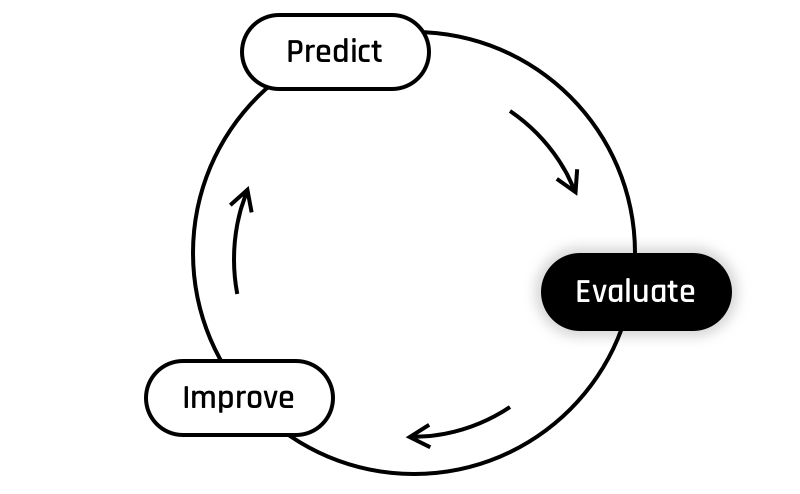
\includegraphics[scale=0.25]{assets/Evaluate.png}
  % \caption{cycle evaluate}
\end{figure}

\subsection*{Introducing the loss function}

How good is our model?  
It is hard to say just by simply looking at the plots!
We can clearly observe that certain regression lines seem to fit the data better than others, but it would be convenient to find a way to measure it. 

\begin{figure}[h!]
  \centering
  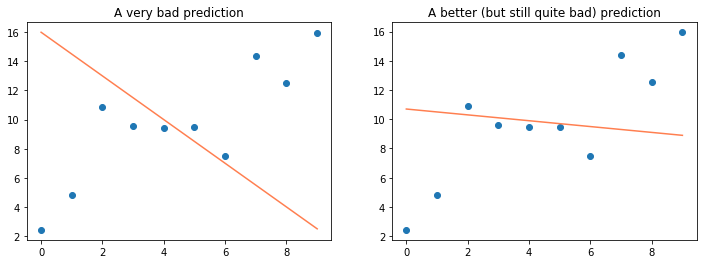
\includegraphics[scale=0.55]{assets/bad_prediction.png}
  \caption{bad prediction}
\end{figure}

To evaluate our model, we are going to use a \textbf{metric} called \textbf{the loss function} (sometimes called \textbf{cost function}).\\
\newline
The loss function tells us how bad our model is performing, how much it \textit{costs} us to use it, how much information we \textit{lose} when we use it.
If the model is good, we won't lose that much; if it's terrible instead, we will have a high loss!

The metric you choose will deeply impact the evaluation (and therefore also the training) of your model.

A frequent way to evaluate the performance of a regression model is to measure the distance between each predicted value ($\hat{y}^{(i)}$) and the real value it tries to predict (${y}^{(i)}$). The distances are then squared, and averaged to get one single metric, denoted $J$:

$$
J(\theta) = \frac{1}{2m}\sum_{i=1}^{m}(\hat{y}^{(i)} - y^{(i)})^2
$$

The smaller, the better! 

\begin{figure}[h!]
  \centering
  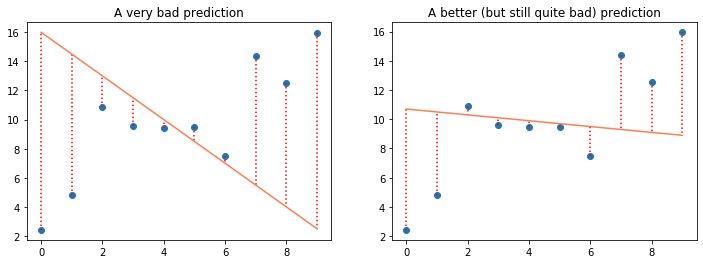
\includegraphics[scale=0.55]{assets/bad_pred_with_distance.png}
  \caption{bad prediction with distance}
\end{figure}

\newpage
\turnindir{ex06}
\exnumber{06}
\exfiles{ridge.py}
\exforbidden{sklearn}
\makeheaderfilesforbidden

% ================================= %
\section*{Objective}
% --------------------------------- %
Now it's time to implement your \texttt{MyRidge} class, similar to the class of the same name in \texttt{sklearn.linear\_model}.

% ================================= %
\section*{Instructions}
% --------------------------------- %
In the \texttt{ridge.py} file, create the following class as per the instructions given below:

Your \texttt{MyRidge} class will have at least the following methods:
\begin{itemize}
  \item \texttt{\_\_init\_\_}, special method, similar to the one you wrote in \texttt{MyLinearRegression} (module06),
  \item \texttt{get\_params\_}, which get the parameters of the estimator, 
  \item \texttt{set\_params\_}, which set the parameters of the estimator,
  \item \texttt{loss\_}, which return the loss between 2 vectors (numpy arrays),
  \item \texttt{loss\_elem\_}, which return a vector corresponding to the squared diffrence between 2 vectors (numpy arrays),  
  \item \texttt{predict\_}, which generates predictions using a linear model,
  \item \texttt{gradient\_}, which calculates the vectorized regularized gradient,
  \item \texttt{fit\_}, which fits Ridge regression model to a training dataset.
\end{itemize}

\hint{
  You should consider inheritance from \texttt{MyLinearRegression}.
}
If \texttt{MyRidge} inheritates from \texttt{MyLinearRegression}, you may not need to reimplement \texttt{predict\_} method.

The difference between \texttt{loss\_elem\_}, \texttt{loss\_}, \texttt{gradient\_} and \texttt{fit\_} methods implementation \texttt{MyRidge}'s and \texttt{MyLinearRegression} (implemented in module 02) is the use of a regularization term.

\begin{minted}[bgcolor=darcula-back,formatcom=\color{lightgrey},fontsize=\scriptsize]{python}
class MyRidge(ParentClass):
	"""
	Description:
		My personnal ridge regression class to fit like a boss.
	"""
	def __init__(self,  thetas, alpha=0.001, max_iter=1000, lambda_=0.5):
		self.alpha = alpha
		self.max_iter = max_iter
		self.thetas = thetas
		self.lambda_ = lambda_
		... Your code here ...

	... other methods ...
\end{minted}

\hint{
  again, this is a good use case for decorators...
}

% ===========================(fin ex 06)         %
% ============================================== %

\newpage

% ============================================== %
% ===========================(start ex 07)       %
\chapter{Exercise 07}
\extitle{Practicing Ridge Regression}
%%******************************************************************************%
%                                                                              %
%                                 Interlude                                    %
%                         for Machine Learning module                          %
%                                                                              %
%******************************************************************************%

% =============================================== %
\section*{Interlude - Introducing Polynomial Models}
% ----------------------------------------------- %

You probably noticed that the method we use is called \textit{linear regression} for a reason:
the model generates all of its predictions on a straight line.
However, we often encounter features that do not have a linear relationship with the predicted variable,
like in the figure below:

\begin{figure}[!h]
    \centering
    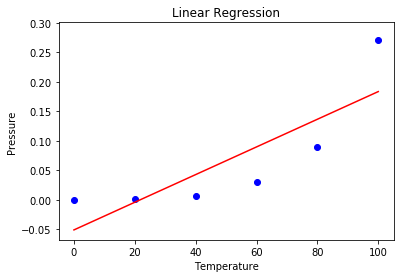
\includegraphics[scale=0.6]{assets/polynomial_straight_line.png}
    \caption{Non-linear relationship}
\end{figure}

In that case, we are stuck with a straight line that cannot fit the data points properly.
In this example, what if we could express $y$ not as a function of $x$, but also of $x^2$, and maybe even $x^3$ and $x^4$?
We could make a hypothesis that draws a nice \textbf{curve} that would better fit the data.
That's where polynomial features can help!

% =============================================== %
\section*{Interlude - Polynomial features}
% ----------------------------------------------- %
First we get to do some \textit{feature engineering}.
We create new features by raising our initial $x$ feature to the power of 2, and then 3, 4... as far as we want to go.
For each new feature we need to create a new column in the dataset.

% =============================================== %
\section*{Interlude - Polynomial Hypothesis}
% ----------------------------------------------- %
Now that we created our new features, we can combine them in a linear hypothesis that looks just the same as what we're used to:

$$
\hat{y} = \theta_0 + \theta_1 x  +\theta_2 x^{2} + \dots + \theta_n x^{n}
$$  

It's a little strange because we are building a linear combination, not with different features but with different powers of the same feature.
This is a first way of introducing non-linearity in a regression model!
%\newpage
\turnindir{ex07}
\exnumber{07}
\exfiles{space\_avocado.py, benchmark\_train.py,  models.[csv/yml/pickle]}
\exforbidden{sklearn}
\makeheaderfilesforbidden


% ================================= %
\section*{Objective}
% --------------------------------- %
It's training time!  
Let's practice our brand new Ridge Regression with a polynomial model.

% ================================= %
\section*{Introduction}
% --------------------------------- %
You have already used the dataset \texttt{space\_avocado.csv}.
The dataset is constituted of 5 columns:
\begin{itemize}
  \item \textbf{index}: not relevant,
  \item \textbf{weight}: the avocado weight order (in ton),
  \item \textbf{prod\_distance}: distance from where the avocado ordered is produced (in Mkm),
  \item \textbf{time\_delivery}: time between the order and the receipt (in days),
  \item \textbf{target}: price of the order (in trantorian unit).
\end{itemize}
It contains the data of all the avocado purchase made by Trantor administration (guacamole is a serious business there).

% ================================= %
\section*{Instructions}
% --------------------------------- %
You have to explore different models and select the best you find.
To do this:
\begin{itemize}
  \item Split your \texttt{space\_avocado.csv} dataset into a training, a cross-validation and a test sets.
  \item Use your \texttt{polynomial\_features} method on your training set.
  \item Consider several Linear Regression models with polynomial hypotheses with a maximum degree of $4$.
  \item For each hypothesis consider a regularized factor ranging from $0$ to $1$ with a step of $0.2$.
  \item Evaluate your models on the cross-validation set.
  \item Evaluate the best model on the test set.
\end{itemize}

According to your model evaluations, what is the best hypothesis you can get?
\begin{itemize}
  \item Plot the evaluation curve which help you to select the best model (evaluation metrics vs models + $\lambda$ factor).
  \item Plot the true price and the predicted price obtain via your best model with the different $\lambda$ values (meaning the dataset + the 5 predicted curves).
\end{itemize}


The training of all your models can take a long time.
Thus you need to train only the best one during the correction.
But, you should return in \texttt{benchmark\_train.py} the program which perform the training of all the models and save the parameters of the different models into a file.
In \texttt{models.[csv/yml/pickle]} one must find the parameters of all the models you have explored and trained.
In \texttt{space\_avocado.py} train the model based on the best hypothesis you find and load the other models from \texttt{models.[csv/yml/pickle]}.
Then evaluate the best model on the right set and plot the different graphics as asked before.

% ===========================(fin ex 07)         %
% ============================================== %

\newpage

% ============================================== %
% ===========================(start ex 08)       %
\chapter{Exercise 08}
\extitle{Regularized Logistic Regression}
%******************************************************************************%
%                                                                              %
%                                 Interlude                                    %
%                         for Machine Learning module                          %
%                                                                              %
%******************************************************************************%

\section*{Interlude - Fifty Shades of Linear Algebra}

In the last exercise, we implemented the loss function in two subfunctions.
It worked, but it's not very pretty.
What if we could do it all in one step, with linear algebra?   

As we did with the hypothesis, we can use a vectorized equation to improve the calculations of the loss function.

So now let's look at how squaring and averaging can be performed (more or less) in a single matrix multiplication!

$$
J(\theta) = \frac{1}{2m}\sum_{i=1}^{m}(\hat{y}^{(i)} - y^{(i)})^2
$$
$$
J(\theta) = \frac{1}{2m}\sum_{i=1}^{m}[(\hat{y}^{(i)} - y^{(i)}) (\hat{y}^{(i)} - y^{(i)})]
$$

Now, if we apply the definition of the dot product:

$$
J(\theta) = \frac{1}{2m}(\hat{y} - y) \cdot(\hat{y}- y)
$$
\newpage
\turnindir{ex08}
\exnumber{08}
\exfiles{my\_logistic\_regression.py}
\exforbidden{sklearn}
\makeheaderfilesforbidden

% ================================= %
\section*{Objective}
% --------------------------------- %
In the last exercise, you implemented of a regularized version of the linear regression algorithm, called Ridge regression.
Now it's time to update your logistic regression classifier as well!
In the \texttt{scikit-learn} library, the logistic regression implementation offers a few regularization techniques, which can be selected using the parameter \texttt{penalty} (L$_2$ is default).
The goal of this exercise is to update your old \texttt{MyLogisticRegression} class to take that into account.

% ================================= %
\section*{Instructions}
% --------------------------------- %
In the \texttt{my\_logistic\_regression.py} file, update your \texttt{MyLogisticRegression} class according to the following:

\begin{itemize}
  \item \textbf{add} a \texttt{penalty} parameter which can take the following values:\texttt{'l2'}, \texttt{'none'} (default value is \texttt{'l2'}).
\end{itemize}
\begin{minted}[bgcolor=darcula-back,formatcom=\color{lightgrey},fontsize=\scriptsize]{python}
class MyLogisticRegression():
	"""
	Description:
		My personnal logistic regression to classify things.
	"""
  supported_penalities = ['l2'] # We consider l2 penality only. One may wants to implement other penalities

	def __init__(self, theta, alpha=0.001, max_iter=1000, penality='l2', lambda_=1.0):
		# Check on type, data type, value ... if necessary
    self.alpha = alpha
		self.max_iter = max_iter
		self.theta = theta
		self.penality = penality
    self.lambda_ = lambda_ if penality in self.supported_penalities else 0
		#... Your code ...

	... other methods ...
\end{minted}

\begin{itemize}
  \item \textbf{update} the \texttt{fit\_(self, x, y)} method: 
  \begin{itemize}
    \item \texttt{if penality == 'l2'}: use a \textbf{regularized version} of the gradient descent.
    \item \texttt{if penality = 'none'}: use the \textbf{unregularized version} of the gradient descent from \texttt{module03}.
  \end{itemize}
\end{itemize}

% ================================= %
\section*{Examples}
% --------------------------------- %
\begin{minted}[bgcolor=darcula-back,formatcom=\color{lightgrey},fontsize=\scriptsize]{python}
from my_logistic_regression import MyLogisticRegression as mylogr

theta = np.array([[-2.4], [-1.5], [0.3], [-1.4], [0.7]])

# Example 1:
model1 = mylogr(theta, lambda_=5.0)

model1.penality
# Output
'l2'

model1.lambda_
# Output
5.0

# Example 2:
model2 = mylogr(theta, penality=None)

model2.penality
# Output
None

model2.lambda_
# Output
0.0

# Example 3:
model3 = mylogr(theta, penality=None, lambda_=2.0)

model3.penality
# Output
None

model3.lambda_
# Output
0.0

\end{minted}

\hint{
  this is also a great use case for decorators...
}

% ===========================(fin ex 08)         %
% ============================================== %

\newpage

% ============================================== %
% ===========================(start ex 09)       %
\chapter{Exercise 09}
\extitle{Practicing Regularized Logistic Regression}
%%******************************************************************************%
%                                                                              %
%                                 Interlude                                    %
%                         for Machine Learning module                          %
%                                                                              %
%******************************************************************************%

% ============================================== %
\section*{Interlude - Lost in Overfitting}
% ---------------------------------------------- %

The two previous exercises lead you, dear reader, to a very dangerous territory: the realm of \textbf{overfitting}.\\
You did not see it coming but now, you are in a bad situation...\\
\\
By increasing the polynomial degree of your model, you increased its \textbf{complexity}.  
Is it wrong?
Not always.
Some models are indeed very complex because the relationships they represent are very complex as well.\\
\\
But, if you look at the plots for the previous exercise's \textit{best model}, you should feel that something is wrong...\\
\\
% ============================================== %
\section*{Interlude - Something is rotten in the state of our model...}
% ---------------------------------------------- %
Take a look at the following plot. 

\begin{figure}[!h]
    \centering
    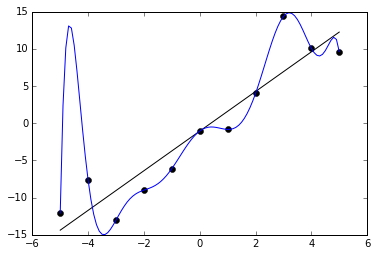
\includegraphics[scale=0.6]{assets/overfitt.png}
    \caption{Overfitting hypothesis}
\end{figure}

You can see that the prediction line fits each data point perfectly, but completely misses out on capturing the relationship between $x$ and $y$ properly.
And now, if we add some brand new data points to the dataset, we see that the predictions on those new examples are way off.

\begin{figure}[!h]
    \centering
    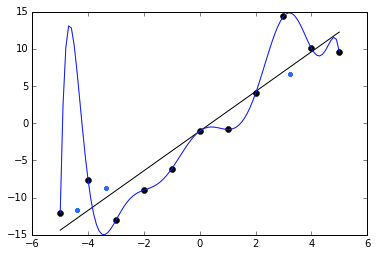
\includegraphics[scale=0.6]{assets/overfitt_with_dots.png}
    \caption{Generalization errors resulting from overfitting}
\end{figure}
This situation is called overfitting, because the model is doing an excessively good job at fitting the data.
It is literally bending over backward to account for the data's mini details.
But most of the data's irregularities are just noise, and they should in fact be ignored.
So because the model overfits, it can't generalize to new data.

% ============================================== %
\section*{Interlude - The training set, the test set, and the happy data scientist}
% ---------------------------------------------- %
To be able to detect overfitting, \textbf{you should always evaluate your model on new data}.\\
\\
New data means, data that your model hasn't seen during training.\\
\\
It's the only way to make sure your model isn't \textit{recalling}.
To do so, now and forever, you must always divide your dataset in (at least) two parts: one for the training, and one for the evaluation of your model.
%\newpage
\turnindir{ex09}
\exnumber{09}
\exfiles{solar\_system\_census.py, benchmark\_train.py,  models.[csv/yml/pickle]}
\exforbidden{sklearn}
\makeheaderfilesforbidden

% ================================= %
\section*{Objective}
% --------------------------------- %
It's training time!
Let's practice our updated Logistic Regression with polynomial models.
% ================================= %
\section*{Introduction}
% --------------------------------- %
You have already used the dataset \texttt{solar\_system\_census.csv} and \texttt{solar\_system\_census\_planets.csv}.
\begin{itemize}
	\item The dataset is divided in two files which can be found in the \texttt{resources} folder: \texttt{solar\_system\_census.csv} and \texttt{solar\_system\_census\_planets.csv}.
	\item The first file contains biometric information such as the height, weight, and bone density of several Solar System citizens.
	\item The second file contains the homeland of each citizen, indicated by its Space Zipcode representation (i.e. one number for each planet... :)).  
\end{itemize}

As you should know, Solar citizens come from four registered areas (zipcodes): 

\begin{itemize}
	\item The flying cities of Venus ($0$), 
	\item United Nations of Earth ($1$), 
	\item Mars Republic ($2$), 
	\item The Asteroids' Belt colonies ($3$).
\end{itemize}

% ================================= %
\section*{Instructions}
% --------------------------------- %
% ================================= %
\subsection*{Split the Data}
% --------------------------------- %

Take your \texttt{solar\_system\_census.csv} dataset and split it in a \textbf{training set}, a \textbf{cross-validation set}
and  a \textbf{test set}.

% ================================= %
\subsection*{Training and benchmark}
% --------------------------------- %
One part of your submission will be find in \texttt{benchmark\_train.py} and \texttt{models.[csv/yml/pickle]} files.
You have to:
\begin{itemize}
  \item Train different regularized logistic regression models with a polynomial hypothesis of \textbf{degree 3}.
        The models will be trained with different $\lambda$ values, ranging from $0$ to $1$.
        Use one-vs-all method.
  \item Evaluate the \textbf{f1 score} of each of the models on the cross-validation set.
        You can use the \texttt{f1\_score\_} function that you wrote in the \texttt{ex11} of \texttt{module08}.
  \item Save the different models into a \texttt{models.[csv/yml/pickle]}.
\end{itemize}

% ================================= %
\subsection*{Solar system census program}
% --------------------------------- %
The second and last part of your submission is in \texttt{solar\_system\_census.py}. You have to:
\begin{itemize}
  \item Loads the differents models from \texttt{models.[csv/yml/pickle]} and train from scratch only the best one on a training set.
  \item Visualize the performance of the different models with a bar plot showing the score of the models given their $\lambda$ value.
  \item Print the \textbf{f1 score} of all the models calculated on the test set.
  \item Visualize the target values and the predicted values of the best model on the same scatterplot. Make some effort to have a readable figure.
\end{itemize}

\info{For the second script \texttt{solar\_system\_census.py}, only a train and test set are necessary as one is simply looking to the performance.}

% ===========================(fin ex 09)         %
% ============================================== %

\newpage

% ============================================== %
% ===========================(Conclusion)        %
\chapter{Conclusion - What you have learnt}

The excercises serie is finished, well done!
Based on all the knowledges tackled today, you should be able to discuss and answer the following questions:

\begin{enumerate}
  \item Why do we use logistic hypothesis for a classfication problem rather than a linear hypothesis?
  \item What is the decision boundary?
  \item In the case we decide to use a linear hypothesis to tackle a classification problem, why the classification of some data points can be modified by considering more examples (for example, extra data points with extrem ordinate)?
  \item In a one versus all classification approach, how many logisitic regressor do we need to distinguish between N classes?
  \item Can you explain the difference between accuracy and precision? What is the type I and type II errors?
  \item What is the interest of the F1-score?
\end{enumerate}

% ===========================(Conclusion)        %
% ============================================== %

\newpage

% ================================= %
\section*{Contact}
% --------------------------------- %
You can contact 42AI association by email: contact@42ai.fr\\
You can join the association on \href{https://join.slack.com/t/42-ai/shared_invite/zt-ebccw5r7-YPkDM6xOiYRPjqJXkrKgcA}{42AI slack}
and/or posutale to \href{https://forms.gle/VAFuREWaLmaqZw2D8}{one of the association teams}.

% ================================= %
\section*{Acknowledgements}
% --------------------------------- %
The modules Python \& ML is the result of a collective work, we would like to thanks:
\begin{itemize}
  \item Maxime Choulika (cmaxime),
  \item Pierre Peigné (ppeigne),
  \item Matthieu David (mdavid),
  \item Quentin Feuillade--Montixi (qfeuilla, quentin@42ai.fr)
\end{itemize}
who supervised the creation, the enhancement and this present transcription.

\begin{itemize}
  \item Louis Develle (ldevelle, louis@42ai.fr)
  \item Owen Roberts (oroberts)
  \item Augustin Lopez (aulopez)
  \item Luc Lenotre (llenotre)
  \item Amric Trudel (amric@42ai.fr)
  \item Benjamin Carlier (bcarlier@student.42.fr)
  \item Pablo Clement (pclement@student.42.fr)
\end{itemize}
for your investment for the creation and development of these modules.

\begin{itemize}
  \item Richard Blanc (riblanc@student.42.fr)
  \item Solveig Gaydon Ohl (sgaydon-@student.42.fr)
  \item Quentin Feuillade Montixi (qfeuilla@student.42.fr)
\end{itemize}
who betatest the first version of the modules of Machine Learning.
\vfill
\doclicenseThis
\end{document}
